\documentclass{IJFS}



\usepackage{amsfonts,amsthm,amsmath,amssymb,dsfont}
\usepackage{amsmath,    enumitem}
\usepackage{graphicx}
\usepackage{color}
%\usepackage[colorlinks]{hyperref}
\usepackage[all]{xy}
\usepackage{subfigure}
\usepackage{tikz}
\usetikzlibrary[arrows,shapes,graphs,decorations.pathmorphing,backgrounds,positioning,fit,petri]
\usepackage{ amscd,   eufrak}

 \usepackage{amssymb}
 \usepackage{amsmath}
 
 \usepackage{mathrsfs}
 \usepackage{amsfonts}

 \usepackage{verbatim}

\usepackage{epstopdf}% To incorporate .eps illustrations using PDFLaTeX, etc.
\usepackage{subfigure}% Support for small, `sub' figures and tables
\usepackage[latin1]{inputenc}
\usepackage{tikz}
\usetikzlibrary{shapes,arrows}
\usepackage[numbers,sort&compress]{natbib}% Citation support using natbib.sty
\bibpunct[, ]{[}{]}{,}{n}{,}{,}% Citation support using natbib.sty
\renewcommand\bibfont{\fontsize{10}{12}\selectfont}% Bibliography support using natbib.sty
\usepackage{rotating}

\newtheorem{theorem}{Theorem}[section]
\newtheorem{lemma}[theorem]{Lemma}
\newtheorem{proposition}[theorem]{Proposition}
\newtheorem{corollary}[theorem]{Corollary}
\newtheorem{notation}[theorem]{Notation}
\newtheorem{definition}[theorem]{Definition}
\newtheorem{ex}[theorem]{Example}
\newtheorem{remark}[theorem]{Remark}


 \def\dis{\displaystyle}
 
\begin{document}

\tikzstyle{decision} = [diamond, draw, fill=orange!20, 
text width=6em, text badly centered, node distance=3cm, inner sep=0pt]
\tikzstyle{block} = [rectangle, draw, fill=orange!20, 
text width=9em, text centered, rounded corners, minimum height=4em]
\tikzstyle{block2} = [rectangle, draw, fill=orange!20, 
text width=9em, text centered, rounded corners, minimum height=4em]
\tikzstyle{line} = [draw, -latex']
\tikzstyle{cloud} = [draw, ellipse,fill=red!20, node distance=3cm,
minimum height=4em]

\addtocounter{page}{0}

\titleijfs{Spherical Fuzzy Soft Sets: Theory and Aggregation Operator with its Applications}

\author[1]{E. G\"{u}ner} 
\author[1]{H.
Ayg\"{u}n}
\affil[1]{Department of Mathematics, Kocaeli University, Umuttepe Campus, 41380, Kocaeli, Turkey}


\emails{elif.guner@kocaeli.edu.tr, halis@kocaeli.edu.tr}

\CorrespondAuthor{E. G\"{u}ner}

\oddPageHead{Spherical Fuzzy Soft Sets: Theory and Aggregation Operator with its Applications}
\evenPageHead{E. G\"{u}ner, H.
Ayg\"{u}n}

\abstractijfs{
The aim of this paper is to redefine the notion of spherical fuzzy soft sets as a more general concept to make them more functional for solving multi-criteria decision-making problems.
We first define the set operations under the new spherical fuzzy soft set environment and obtain some fundamental properties of them.
Then, we construct the spherical fuzzy soft aggregation operator which allows establishing a more efficient and useful method to solve the multi-criteria decision-making problems. We establish an algorithm for the decision-making process which is more useful, simple, and easier than the existing methods.
After constructing the method for solving the decision-making problem, we give a numerical example based on linguistic terms to show that the validity of the proposed technique.
Finally, we analyze the reliability of the results of this method with the help of the comparative studies by applying this to a real-time data set and using the existing methods.
}

\keywords_ijfs{Spherical fuzzy sets, spherical fuzzy soft
sets, aggregation operator, multi-criteria decision-making problem.
\vspace{1mm}\\
{\it 2010 MSC}: 03E72, 91B06, 93B28.
}

\Vol{*}	\No{*}	\Year{****}	\Pages{**}
\Received{**}	\Revised{**}		\Accepted{**}

{\let\newpage\relax\vspace*{.1mm}
\noindent\rule{\textwidth}{.3mm}\maketitle}

\thispagestyle{fancylogo}

\mabstract


\section{ Introduction}
As we all know, since the fuzzy set theory has been introduced in 1965 by Zadeh detailed in \cite{zadeh}, many researchers have concentrated on this theory by applying this theory to different fields of science such that image processing, data mining, engineering, medical sciences, clustering, statistical information theory and etc. But since a fuzzy set has only a membership (positive-membership) degree, it has some restrictions in expressing uncertain data. For this reason, the fuzzy set has been extended to many new types of fuzzy sets in various consideration: Type-2 fuzzy sets by Zadeh \cite{zadeh1}; Interval-valued fuzzy sets by Sambuc \cite{sam}, Zadeh, Jahn and Grattan-Guinness; Intuitionistic fuzzy sets by Atanassov \cite{ata}; Fuzzy multi-sets by Yager \cite{yager}; Neutrosophic sets by Smarandache \cite{sma}; Non-stationary fuzzy sets by Garibaldi and Ozen \cite{gari}; Hesitant fuzzy sets by Torra \cite{tor}; Pythagorean fuzzy sets by Yager \cite{yager1}; Picture fuzzy sets by Cuong \cite{cuon} and Spherical fuzzy sets by Kahraman and Kutlu G\"{u}ndo\u gdu \cite{kut0}.

Another extension of the fuzzy set theory is the soft set theory introduced by Molodtsov \cite{mol} to deal with the uncertainties and vagueness  of many problems that arise in medical science,
engineering, social science,  economics and etc. This theory has been studied in various areas with significant applications (see \cite{aa, cet,2s,  maji, pazar}). After, with the combination of the
extension of fuzzy sets which are mentioned above and soft sets, many different set theories have been obtained: Fuzzy soft sets by Maji et al. \cite{maji1} and \c{C}agman et al. \cite{cag}; Intuitionistic fuzzy soft sets by \c{C}agman and Karata\c s \cite{cag1}; Hesitant fuzzy soft sets by Babitha and John
\cite{babit}; Pythagorean fuzzy soft sets by Peng et al. \cite{peng}; Picture fuzzy soft sets by Yang et al. \cite{yang}; Spherical fuzzy soft sets by Perveen et al. \cite{per}.

If we return to the real-life, the work of scientists, managers, lawyers, engineers that steers the course of society is largely making decisions and solving problems. Decision-making is very
important not only mentioned at the level of business organizations but also at the level of our individual lives (buying a house, choosing a school or a career). During the past half-century, major research gains have been made in understanding problem-solving and decision making in many fields such as
psychology, economics, mathematical statistics, operations research, political science, artificial intelligence, and cognitive science. In a lot of decision-making problems, we may face various types of uncertainties. To handle these situations, appropriate sets of data and methods have been used by following the developments in science. The first application of the fuzzy set theory to decision-making problems was given by Bellman and Zadeh \cite{bel} in 1970. After this paper, a lot of studies have been made with two types of methods, one is the traditional decision-making methods such as AHP, VIKOR, WASPAS and another is established on some operators which aggregate the information. In the point of aggregation operators, many theories and applications were improved in recent years by considering the new types of fuzzy sets: For instance, Xu \cite{xu} presented the arithmetic weighted aggregation operators for intuitionistic fuzzy numbers. Wei \cite{wei, wei1} utilized arithmetic and geometric operations to develop some picture fuzzy aggregation operators, also proposed picture fuzzy Hamacher aggregation operators and picture fuzzy Hamacher geometric aggregation operators with applications to enterprise resource planning.  Ashraf and Abdullah \cite{as2} extended different strict Archimedean triangular norms and triangular conorms to aggregate the spherical fuzzy information and also defined some spherical aggregation operators and applied these operators to multi-criteria group decision-making problems. Different types of aggregation operators for spherical fuzzy sets can be found in \cite{as3, gun, jin, mah, wan}. The traditional decision-making methods in spherical fuzzy environment was given in \cite{ kutlu, kutlu1, kutlu2}.  Yang et al. \cite{yang} introduced an algorithm based on adjustable soft discernibility matrix by using the level soft set of a picture fuzzy soft set to solve decision-making problems, which can find an order relation of all the objects. Perveen et al.  \cite{per} proposed an algorithm based on adjustable soft discernibility matrix to solve the decision-making problem in spherical fuzzy soft environment. Guleria and Bajaj \cite{gul} initiated some aggregation operators to merge the spherical fuzzy soft information. Ahmmad et al. \cite{ah} presented some average aggregation operators in spherical fuzzy soft environment and their applications in multi-criteria decision process.

In the present work, we redefine the notion of spherical fuzzy soft sets as a more general concept from the definition of \cite{per} to make them more functional and efficient when solving multi-criteria decision-making problems. The new concept of spherical fuzzy soft sets is larger than the concept of spherical fuzzy soft sets given by Perveen et al. \cite{per}. Also, we initiate the set operations under the spherical fuzzy soft set environment and obtain some fundamental properties of them by defining the null sf-set and universal sf-set. Then, we present the spherical fuzzy soft aggregation operator which allows establishing a more efficient and easier method to solve the multi-criteria decision-making problems. After introducing the notion of spherical fuzzy soft aggregation operators, we propose an algorithm based on linguistic terms that is more useful and practical for the decision-making process than the existing methods. Then, we give a numerical example to clarify the proposed technique. Finally, we compare the results of this method with using a real-time data set and the existing methods.



\section{Preliminaries}
In this section, we yield some fundamental concepts concerned with
soft sets, fuzzy soft sets and spherical fuzzy sets which will be
necessary for the main sections. Throughout this paper, $U$ will
denote an initial universe, $E$ refers to a non-empty parameters
set and suppose that $A \subset E$, unless otherwise specified.


\begin{definition} \cite{mol} A pair $(F,E)$ is called a soft
set (s-set) over $U$ if  $F$ is a mapping of $E$ into the set of all
subsets of the set $U$ (i.e., $F:E\rightarrow \mathscr{P}(U)$).  Every set $F(e)$ for all
$e\in E$, from this family may be considered as the set
of $e-$elements of the soft set $(F,E)$, or as the set
of $e-$approximate elements of the soft set.

\end{definition}

\begin{definition} \cite{maj} Let $I^U$ denote the  family of all fuzzy sets (f-sets) $f:U\to I$. A pair $(F, E)$ is called a fuzzy soft set (fs-set) over $U$ if $F: E\to I^U$ is a function.

Obviously, an  s-set $(F,E)$ over $U$ can be thought as an fs-set by
using the characteristic function of the set $F(e)$:
\begin{center}
    $~~~~~~~~\displaystyle F(e)(a)=
\begin{cases}
\displaystyle 1, &\text{if $a\in F(e)$;}\\
0, &\text{otherwise.}
\end{cases}$
\end{center}

\end{definition}

\begin{definition} \cite{as00,cuon, kut0} Let $\mu:U\to [0,1]$, $\iota:U\to [0,1]$ and $\nu:U\to [0,1]$ be three mappings. A set \linebreak[4] $S=\{<u, \mu(u), \iota(u), \nu(u)>|u\in U\}$
is called a

(i) picture fuzzy set (pf-set) over $U$ if   $0\le
\mu(u)+\iota(u)+\nu(u)\le 1$ for all $u\in U$.

(ii) spherical fuzzy set (sf-set) over $U$ if   $0\le
\mu^2(u)+\iota^2(u)+\nu^2(u)\le 1$ for all $u\in U$. 

The values
$\mu(u), \iota(u), \nu(u)\in [0,1]$ denote the degree of
positive-membership, neutral-memberhip and negative-membership of
$u$ to $S$, respectively. We will denote by $PF(U)$ and $SF(U)$ with the set
of all pf-sets and sf-sets over $U$, respectively.

\end{definition}  

\begin{definition} \cite{yang} A pair $(F, E)$ is called a picture fuzzy soft set (pfs-set) over $U$ if $F: E\to PF(U)$ is a function.

\end{definition}

\begin{remark}
It is clear that the family of all sf-sets over $U$ contains the family of all pf-set over $U$ and the family of all pf-set over contains the family of all $U$ f-sets over $U$. Also,  the family of  pfs-sets over $U$  contains the family of all fs-sets over $U$ and the family of  fs-sets over $U$  contains the family of all s-sets over $U$.
\end{remark}

We give the definitions of null sf-set and universal sf-set similar to the f-sets as follows: 
\begin{definition} Let $S\in SF(U)$.

(1) $S$ is said to be a null sf-set denoted by $\bar{0}$ if
$S=\{<u,0,0,1>:u\in U\}$.

(2) $S$ is said to be a universal sf-set denoted by $\bar{U}$ if
$S=\{<u,1,0,0>:u\in U\}$.
\end{definition}

The set operations under sf-sets are given by Ashraf et al. \cite{as00} as follows:

\begin{definition}\cite{as00} For the sf-sets $S_1=\{<u,\mu_1(u), \iota_1(u),\nu_1(u)>:u\in U\}$ and  $S_2=\{<u, \mu_2(u), \iota_2(u), \nu_2(u)>:u\in U\}$, the set operations are
defined as follows:

(1) $S_1 \sqsubseteq S_2$ if $\mu_1(u)\le \mu_2(u)$,
$\iota_1(u)\le \iota_2(u)$ and $\nu_1(u)\ge \nu_2(u)$ for all
$u\in U$.

(2) $S_1=S_2$ if and only if $S_1\sqsubseteq S_2$ and $S_2
\sqsubseteq S_1$.

(3) The union of $S_1$ and $S_2$ is denoted by $S_1 \sqcup S_2$ and defined by \linebreak[4] $S_1 \sqcup S_2=\{<u,max\{\mu_1(u),\mu_2(u)\}, min\{\iota_1(u), \iota_2(u)\}, min\{\nu_1(u), \nu_2(u)\}>:u\in
U\}$.

(4) The intersection of $S_1$ and $S_2$ is denoted by $S_1 \sqcap
S_2$ and defined by \linebreak[4] $S_1 \sqcap S_2=\{<u,min\{\mu_1(u),\mu_2(u)\},
min\{\iota_1(u), \iota_2(u)\}, max\{\nu_1(u), \nu_2(u)\}>:u\in
U\}$.
\end{definition}

\begin{lemma} (i) $\bar{0} \sqsubseteq S$ for all $S\in SF(U)$.

(ii) $ S \sqsubseteq \bar{U}$ for all $S\in SF(U)$.

(iii) $S \sqcup \bar{U}=\bar{U}$ for all $S\in SF(U)$.

(iv) $S \sqcap \bar{0}=\bar{0}$ for all $S\in SF(U)$.

\end{lemma}

\begin{definition} \cite{as0} Let $S\in SF(U)$ where $S=\{<u, \mu(u), \iota(u), \nu(u)>|u\in U\}$. Then  the complement of $S$ is denoted by $S^c$ and defined
by $S^c=\{<u, \nu(u), \iota(u), \mu(u)>|u\in U\}$. \end{definition}

\begin{remark} Let $S\in SF(U)$. Then $S {\sqcup}S^c\ne \bar{S}$
and $S{\sqcap}S^c\ne \bar{0}$.\end{remark}

The following example is given to illustrate the above remark:
\begin{ex} Let $U=\{u_1, u_2\}$ and $S=\{<u_1, 0.2, 0.3,
0.1>,<u_2, 0.5, 0.3, 0.8>\}$. Then, we obtain the followings 
\begin{eqnarray*}
S^c&=&\{<u_1,
0.1, 0.3, 0.2>, <u_2, 0.8, 0.3, 0.5>\}\\
S{\sqcup}S^c &=&\{<u_1, 0.2, 0.3, 0.1>, <u_2, 0.8, 0.3, 0.5>\}\\
S{\sqcap}S^c &=&\{<u_1, 0.1, 0.3, 0.2>, <u_2, 0.5, 0.3, 0.8>\}
\end{eqnarray*}
which mean that $S{\sqcup}S^c\ne \bar{S}$ and $S{\sqcap}S^c\ne
\bar{0}$.
\end{ex}

The following definitions are recollected to use for solving multi-criteria decision-making problems as seen in the last sections.

\begin{definition} Let  $S\in SF(U)$ where $S=\{<u, \mu(u), \iota(u), \nu(u)>|u\in U\}$. The triplet  $<\mu(u), \iota(u),
\nu(u)>$ is called a $u-element$ of the sf-set $S$. For
simplicity, if $\mu,\iota, \nu \in [0,1]$ and
$\mu^2+\iota^2+\nu^2\le 1$, then the triplet $<\mu,\iota, \nu>$
denotes a spherical fuzzy number (sf-number). We will denote by
$SFN(U)$ with the set of all sf-numbers over $U$.
\end{definition}

\begin{definition} \cite{as00}
Let $S=<\mu, \iota,\nu>, S_1=<\mu_1,\iota_1,\nu_1>$ and
$S_2=<\mu_2,\iota_2,\nu_2>$ be three sf-numbers and $a\ge0$. Then
the operations are defined over the sf-numbers as follows:

(i) $S_1 \oplus S_2=<\sqrt{\mu_1^2+\mu_2^2-\mu_1^2\mu_2^2},
\iota_1\iota_2,\nu_1\nu_2>$,

(ii) $S_1 \odot S_2=<\mu_1\mu_2,
\iota_1\iota_2,\sqrt{\nu_1^2+\nu_2^2-\nu_1^2\nu_2^2}>$,

(iii) $aS=<\sqrt{1-(1-\mu^2)^a},\iota^{a},\nu^{a}>$,

(iv) ${S^a}<\mu^{a}, \iota^{a},\sqrt{1-(1-\nu^2)^a}>$.
\end{definition}


\begin{definition} \cite{as00} Let  $S=<\mu,\iota,\nu>$ be an sf-number.

(i) A score function $SC:SFN(U)\to [0,1]$ is defined as
$SC(S)=\frac{2+\mu-\iota-\nu}{3}$.

(ii) An accuracy function $AC:SFN(U)\to [-1,1]$ is defined as
$AC(S)=\mu-\nu$.
\end{definition}


\begin{definition} \cite{as00} Let  $S_1=<\mu_1,\iota_1,\nu_1>$ and $S_2=<\mu_2,\iota_2,\nu_2>$ be two sf-numbers. Then the ranking method (comparison technique) as
follows:

(i) If $SC(S_1)<SC(S_2)$, then $S_1<S_2$,

(ii) If $SC(S_1)>SC(S_2)$, then $S_1>S_2$,

(iii) $SC(S_1)=SC(S_2)$, then

~~~ (a) $AC(S_1)<AC(S_2)$, then $S_1<S_2$,

~~~ (b) $AC(S_1)>AC(S_2)$, then $S_1>S_2$,

~~~ (c) $AC(S_1)=AC(S_2)$, then $S_1=S_2$.

\end{definition}


\section{sfs-Sets}
In this section, we redefine the notion of spherical fuzzy soft sets in which the parameters set is crisp and the approximation set is sf-set over $U$  by giving their operations. 
\begin{definition} Let $\delta_A:E \to SF(U)$ be a mapping such
that $\delta_A(e)=\bar{0}$ whenever $e\notin A$. Then the set of
ordered pairs

\begin{center}$\Delta_A=\{(e,\delta_A(e)):e\in E, \delta_A(e)\in SF(U)\}$
\end{center}
is called a spherical fuzzy soft set (sfs-set) over $U$. Here,
$\delta_A$ is called the spherical fuzzy approximation function,
$\delta_A(e)$ is a spherical fuzzy set called e-element of the
sfs-set $\Delta_A$ and denoted by $\delta_A(e)=\{<u,
\mu_{\delta_A(e)}(u), \iota_{\delta_A(e)}(u),
\nu_{\delta_A(e)}(u)>:u\in U\}$. We will denote by $SFS(U)$ with
the set of all sfs-sets over $U$.


If $U=\{u_1, u_2, ..., u_n\}$, $E=\{e_1, e_2, ..., e_m\}$ and
$A\subset E$, then  $\Delta_A\in SFS(U)$ can be represented by the
following table:
\begin{table}[!h]
\begin{center} 
\begin{tabular}{c|c c  c}\hline
$\Delta_A$ & $e_1$  & \ldots &$e_m$ \\
\hline $u_1$&$<\mu_{\delta_A(e_1)}(u_1),
\iota_{\delta_A(e_1)}(u_1), \nu_{\delta_A(e_1)}(u_1)>$
&\ldots&$<\mu_{\delta_A(e_m)}(u_1), \iota_{\delta_A(e_m)}(u_1),
\nu_{\delta_A(e_m)}(u_1)>$
\\  $u_2$ &$<\mu_{\delta_A(e_1)}(u_2),
\iota_{\delta_A(e_1)}(u_2), \nu_{\delta_A(e_1)}(u_2)>$
&\ldots&$<\mu_{\delta_A(e_m)}(u_2),
\iota_{\delta_A(e_m)}(u_2), \nu_{\delta_A(e_m)}(u_2)>$\\
 \vdots & \vdots&\ldots&\vdots\\  $u_n$ & $<\mu_{\delta_A(e_1)}(u_n),
\iota_{\delta_A(e_1)}(u_n), \nu_{\delta_A(e_1)}(u_n)>$
&\ldots&$<\mu_{\delta_A(e_m)}(u_n),
\iota_{\delta_A(e_m)}(u_n), \nu_{\delta_A(e_m)}(u_n)>$\\
\end{tabular}\end{center}
\end{table}

If $a_{ij}=<\mu_{\delta_A(e_j)}(u_i), \iota_{\delta_A(e_j)}(u_i),
\nu_{\delta_A(e_j)}(u_i)> $ for $i=1,2...,n$ and $j=1,2,...,m$,
then the sfs-set $\Delta_A$ is represented by the following matrix

\begin{equation}\label{m}
\Delta_A=[a_{ij}]_{n\times m}=\left(
\begin{array}{c c c c}
a_{11}&a_{12}&\ldots&a_{1m}  \\
a_{21}&a_{22}&\ldots&a_{2m} \\
\vdots&\vdots&\vdots&\vdots \\
a_{n1}&a_{n2}&\ldots&a_{nm}
\end{array} \right)
\end{equation}
which is called a  matrix form of the sfs-set $\Delta_A$.
\end{definition}

\begin{ex} Let $U=\{u_1, u_2, u_3\}$,  $E=\{e_1, e_2, e_3,
e_4\}$ and $A=\{e_1, e_3, e_4\}$. Take $\delta_A(e_1)=\{<u_1, 0.2,
0.3, 0.5>, <u_2, 1, 0, 0>, <u_3, 0.8, 0.1, 0.5>\}$,
$\delta_A(e_3)=\{<u_1, 0.8, 0.5, 0.4>, <u_2, 0.9, 0.2, 0.1>, <u_3,
0.2, 0.7, 0.8>\}$ and \linebreak[4] $\delta_A(e_4)=\{<u_1, 0.8, 0.4, 0.2>, <u_2,
0.3, 0.5, 0.7>, <u_3, 0.4, 0.5, 0.5>\}$, then the sfs-set
$\Delta_A$ is written as follows:
\begin{eqnarray*}
\Delta_A&=&\{(e_1, \{<u_1, 0.2, 0.3, 0.5>, <u_2, 1, 0, 0>, <u_3,
0.8, 0.1, 0.5>\}), \\
&&(e_2, \{<u_1,0, 0, 1>, <u_2, 0, 0, 1>, <u_3, 0, 0, 1>\}),\\&&
(e_3,\{<u_1, 0.8, 0.5, 0.4>, <u_2, 0.9, 0.2, 0.1>, <u_3, 0.2, 0.7,
0.8>\}),\\ &&(e_4, \{<u_1, 0.8, 0.4, 0.2>, <u_2, 0.3, 0.5, 0.7>,
<u_3, 0.4, 0.5, 0.5>\})\}.
\end{eqnarray*}
The matrix form of the sfs-set $\Delta_A$ is given by
\begin{center}
$M_{\Delta_A}=\left(
\begin{array}{c c c c}
<0.2, 0.3, 0.5> &<0, 0, 1> &<0.8, 0.5,
0.4>&<0.8, 0.4, 0.2>  \\
<1, 0, 0>& <0, 0, 1>&<0.9, 0.2, 0.1>&<0.3, 0.5, 0.7> \\
<0.8, 0.1, 0.5>&<0, 0, 1>&<0.2, 0.7, 0.8>&<0.4, 0.5, 0.5>
\end{array} \right)$.
\end{center}
\end{ex}



\begin{definition} Let $\Delta_A\in SFS(U)$.

(1) $\Delta_A$ is called a null sfs-set denoted by $\Delta_\Phi$
if $\delta_A(e)=\bar{0}$ for all $e\in E$.

(2) $\Delta_A$ is called an A-universal sfs-set denoted by
$\Delta_{\widetilde{A}}$ if $\delta_A(e)=\bar{U}$ for all $e\in
A$. If $A=E$, then  the A-universal sfs-set is called universal
sfs-set and denoted by $\Delta_{\widetilde{E}}$.
\end{definition}




\begin{definition} Let $\Delta_A, \Delta_B \in SFS(U)$. $\Delta_A$
is said to be an sfs-subset of $\Delta_B$ denoted by $\Delta_A
\widetilde{\sqsubseteq} \Delta_B$ if $\delta_A(e) \sqsubseteq
\delta_B(e)$ for all $e\in E$. i.e., $\mu_{\delta_A(e)}(u)\le
\mu_{\delta_(e)}(u)$, $\iota_{\delta_A(e)}(u)\le
\iota_{\delta_B(e)}(u)$ and $\nu_{\delta_A(e)}(u)\ge
\nu_{\delta_B(e)}(u)$ for all $u\in U$.
 $\Delta_A$ and $\Delta_B$ are said
to be sfs-equal denoted by $\Delta_A=\Delta_B$ if $\Delta_A
\widetilde{\sqsubseteq} \Delta_B$ and $\Delta_B
\widetilde{\sqsubseteq} \Delta_A$.
\end{definition}

\begin{proposition} Let $\Delta_A, \Delta_B, \Delta_C \in SFS(U)$. Then
the followings are satisfied:


(i) $\Delta_\Phi \widetilde{\sqsubseteq} \Delta_A$,

(ii) $\Delta_A \widetilde{\sqsubseteq} \Delta_{\widetilde{A}}$,

(iii) $\Delta_{\widetilde{A}} \widetilde{\sqsubseteq}
\Delta_{\widetilde{E}}$,

(iv) If $\Delta_A \widetilde{\sqsubseteq} \Delta_B$ and $\Delta_B
\widetilde{\sqsubseteq} \Delta_B$, then $\Delta_A
\widetilde{\sqsubseteq} \Delta_C$.
\end{proposition}


\begin{definition} \label{c} Let $\Delta_A\in SFS(U)$. The  complement of
$\Delta_A$ is written as  $\Delta_A^c\in SFS(U)$ and defined by \linebreak[4]
$\Delta_A^c=\{(e,\delta_A^c(e)):e\in E, \delta_A^c(e)\in SF(U)\}$
where  $\delta_A^c(e)=(\delta_A(e))^c$ for all $e\in E$.
\end{definition}

\begin{proposition} Let $\Delta_A\in SFS(U)$. Then the followings are
satisfied:

(i) $(\Delta_A^c)^c=\Delta_A$,

(ii) $\Delta_\Phi^c=\Delta_{\widetilde{E}}$.
\end{proposition}

\begin{proof}
The proofs can be easily obtained by using the
spherical fuzzy approximation function of the sfs-sets
$\Delta_\Phi$, $\Delta_A$ and $\Delta_{\widetilde{E}}$.
\end{proof} 

\begin{definition} \label{bk} Let $\Delta_A, \Delta_B\in SFS(U)$.

(1) The union of $\Delta_A$ and  $\Delta_B$ is the sfs-set
$\Delta_C$ defined by its approximation function
such as $\delta_C(e)=\delta_A(e)\sqcup \delta_B(e)$ for all
$e\in E$. We will denote it by $\Delta_C=\Delta_A \widetilde{\sqcup}
\Delta_B$.

(2) The intersection of $\Delta_A$ and  $\Delta_B$ is the sfs-set
$\Delta_C$ defined by its approximation function such as \linebreak[4]
 $\delta_C(e)=\delta_A(e)\sqcap \delta_B(e)$ for all
$e\in E$.  We will denote it by $\Delta_C=\Delta_A \widetilde{\sqcap}
\Delta_B$.
\end{definition}

\begin{proposition} Let $\Delta_A, \Delta_B, \Delta_C \in SFS(U)$. Then
the followings are satisfied:

(i) $\Delta_A \widetilde{\sqcup} \Delta_A=\Delta_A$,

(ii) $\Delta_A \widetilde{\sqcup} \Delta_\Phi=\Delta_A$,

(iii) $\Delta_A \widetilde{\sqcup}
\Delta_{\widetilde{E}}=\Delta_{\widetilde{E}}$,

(iv) $\Delta_A \widetilde{\sqcup} \Delta_B=\Delta_B
\widetilde{\sqcup} \Delta_A$,

(v) $(\Delta_A \widetilde{\sqcup}
\Delta_B)\widetilde{\sqcup}\Delta_C=\Delta_A \widetilde{\sqcup}
(\Delta_B \widetilde{\sqcup} \Delta_C)$,

(vi) $\Delta_A \widetilde{\sqcap} \Delta_A=\Delta_A$,

(vii) $\Delta_A \widetilde{\sqcap} \Delta_\Phi=\Delta_\Phi$,

(viii) $\Delta_A \widetilde{\sqcap}
\Delta_{\widetilde{E}}=\Delta_A$,

(ix) $\Delta_A \widetilde{\sqcap} \Delta_B=\Delta_B
\widetilde{\sqcap} \Delta_A$,

(x) $(\Delta_A \widetilde{\sqcap}
\Delta_B)\widetilde{\sqcap}\Delta_C=\Delta_A \widetilde{\sqcap}
(\Delta_B \widetilde{\sqcap} \Delta_C)$,

(xi) $\Delta_A \widetilde{\sqcup}
(\Delta_B\widetilde{\sqcap}\Delta_C)=(\Delta_A \widetilde{\sqcup}
\Delta_B) \widetilde{\sqcap}
(\Delta_A\widetilde{\sqcup}\Delta_C)$,

(xii) $\Delta_A \widetilde{\sqcap}
(\Delta_B\widetilde{\sqcup}\Delta_C)=(\Delta_A \widetilde{\sqcap}
\Delta_B) \widetilde{\sqcup}
(\Delta_A\widetilde{\sqcap}\Delta_C)$,
\end{proposition}

\begin{proof}  The proofs of these properties can be shown easily
by using Definition \ref{bk}.
\end{proof}
\begin{remark} Let $\Delta_A\in SFS(U)$. Then $\Delta_A\widetilde{\sqcup}\Delta_A^c\ne
\Delta_{\widetilde{E}}$ and
$\Delta_A\widetilde{\sqcap}\Delta_A^c\ne \Delta_\Phi$.\end{remark}

\begin{ex} Let $U=\{u_1, u_2\}$, $E=\{e_1, e_2, e_3\}$ and $A=\{e_1,
e_2\}$. Take the sfs-set \linebreak[4] $\Delta_A=\{(e_1, \{<u_1, 0.1, 0.2,
0.7>,<u_2, 0.8, 0.3, 0.4>\}), (e_2, \{<u_1, 0.5, 0.3, 0.6>, <u_2,
0.7, 0.5, 0.1>\})\}$. Then, we obtain
\begin{eqnarray*}
\Delta_A\widetilde{\sqcup}\Delta_A^c &=&\{(e_1, \{<u_1, 0.7, 0.2,
0.1>, <u_2, 0.8, 0.3, 0.4>\}), (e_2, \{<u_1, 0.6, 0.3, 0.5>, <u_2,
0.7, 0.5, 0.1>\})\}\\
\Delta_A\widetilde{\sqcap}\Delta_A^c &=&\{(e_1, \{<u_1, 0.1, 0.2,
0.7>, <u_2, 0.4, 0.3, 0.8>\}), (e_2, \{<u_1, 0.5, 0.3, 0.6>, <u_2,
0.1, 0.5, 0.7>\})\}.
\end{eqnarray*}
Hence, we see  that $\Delta_A\widetilde{\sqcup}\Delta_A^c\ne
\Delta_{\widetilde{E}}$ and
$\Delta_A\widetilde{\sqcap}\Delta_A^c\ne \Delta_\Phi$.
\end{ex}
\begin{proposition} Let $\Delta_A, \Delta_B, \Delta_C \in SFS(U)$. Then
the followings are satisfied:

(i) $(\Delta_A \widetilde{\sqcup} \Delta_B)^c=\Delta_A^c
\widetilde{\sqcap} \Delta_B^c$,

(ii) $(\Delta_A \widetilde{\sqcap} \Delta_B)^c=\Delta_A^c
\widetilde{\sqcup} \Delta_B^c$.
\end{proposition}


\begin{proof}  (i) For all $e\in E$, we have
\begin{eqnarray*}
\delta_{A\cup
B}^c(e)&=&(\delta_A(e)\sqcup\delta_B(e))^c=\{<u,max\{\mu_{\delta_A(e)},\mu_{\delta_B(e)}\},
min\{\iota_{\delta_A(e)}, \iota_{\delta_B(e)}\},
min\{\nu_{\delta_A(e)}, \nu_{\delta_B(e)}\}>\}^c\\
&=&\{<u,min\{\nu_{\delta_A(e)}, \nu_{\delta_B(e)}\},
min\{\iota_{\delta_A(e)},
\iota_{\delta_B(e)}\},max\{\mu_{\delta_A(e)},\mu_{\delta_B(e)}\}
>\}=\delta_A^c(e)\sqcap \delta_B^c(e)
\end{eqnarray*}
which means that $(\Delta_A \widetilde{\sqcup}
\Delta_B)^c=\Delta_A^c \widetilde{\sqcap} \Delta_B^c$.

(ii) The proof  can be shown similarly to the above.
\end{proof}

\section{Application of the sfs-sets to the multi-criteria decision-making
problems}
\subsection{sfs-Aggregation operators}

In this subsection, we define the spherical fuzzy soft aggregation
operator which allows solving the multi-criteria decision-making problems with an
easier method.
\begin{definition}
Let $\Delta_A \in SFS(U)$. The cardinal set of $\Delta_A$ is
denoted by $c\Delta_A$ and defined by \linebreak[4] $c\Delta_A=\{
<e,\mu_{c\Delta_A}(e), \iota_{c\Delta_A}(e), \nu_{c\Delta_A}(e)>:
e\in E\}$. Here, $c\Delta_A$ is an sf-set over $E$ and the
positive-membership function $\mu_{c\Delta_A}$, the
neutral-membership function $\iota_{c\Delta_A}$ and the
negative-membership function $\nu_{c\Delta_A}$ of $c\Delta_A$ are
defined as follows:
\begin{equation} \label{c1}
\mu_{c\Delta_A}:E\to [0,1],
\mu_{c\Delta_A}(e)=\frac{|\mu_{\delta_A(e)}|}{|U|}
\end{equation}
where $|\mu_{\delta_A(e)}|$ is the scalar cardinality of the f-set $\mu_{\delta_A(e)}$. i.e.,
$|\mu_{\delta_A(e)}|=\sum_{u_i\in U} \mu_{\delta_A(e)}(u_i)$.
\begin{equation} \label{c2}
\iota_{c\Delta_A}:E\to [0,1],
\iota_{c\Delta_A}(e)=\frac{|\iota_{\delta_A(e)}|}{|U|}
\end{equation}
where $|\iota_{\delta_A(e)}|$ is the scalar cardinality of the
f-set $\iota_{\delta_A(e)}$. i.e.,
$|\iota_{\delta_A(e)}|=\sum_{u_i\in U} \iota_{\delta_A(e)}(u_i)$.
\begin{equation} \label{c3}
\nu_{c\Delta_A}:E\to [0,1],
\nu_{c\Delta_A}(e)=\frac{|\nu_{\delta_A(e)}|}{|U|}
\end{equation}
where $|\nu_{\delta_A(e)}|$ is the scalar cardinality of the f-set
$\nu_{\delta_A(e)}$. i.e., $|\nu_{\delta_A(e)}|=\sum_{u_i\in U}
\nu_{\delta_A(e)}(u_i)$.

We will denote by $cSFS(U)$ with the set of all cardinal sets of
the sfs-sets over $U$. It is obvious that $cSFS(U) \subseteq
SFS(E)$.
\end{definition}


\begin{definition} Let $\Delta_A\in SFS(U)$ and $c\Delta_A$ be the cardinal set of
$\Delta_A$. Then the aggregate sf-set of the sfs-set $\Delta_A$ is
denoted by $\Delta_A^*$ and defined by
$\Delta_A^*=\{<u,\mu_{\Delta_A}^*(u), \iota_{\Delta_A}^*(u),
\nu_{\Delta_A}^*(u)>: u\in U\}$. The positive-membership function
$\mu_{\Delta_A}^*$, the neutral-membership function
$\iota_{\Delta_A}^*$ and the negative-membership function
$\nu_{\Delta_A}^*$ of ${\Delta_A}^*$ are defined as follows:
\begin{eqnarray}
\mu_{\Delta_A}^*:U\to[0,1],
\mu_{\Delta_A}^*(u)=\sqrt{1-\prod_{e\in E}
\bigg(1-\mu_{c\Delta_A}^2(e)\mu_{\delta_A(e)}^2(u)\bigg)^{\frac{1}{|E|}}}\\
\iota_{\Delta_A}^*:U\to[0,1],
\iota_{\Delta_A}^*(u)=\Big(\prod_{e\in E}
\iota_{c\Delta_A}(e)\iota_{\delta_A(e)}(u)\Big)^{\frac{1}{|E|}}\\
\nu_{\Delta_A}^*:U\to[0,1], \nu_{\Delta_A}^*(u)=\Big(\prod_{e\in
E}
\sqrt{{\nu_{c\Delta_A}(e)}^2+{\nu_{\delta_A(e)}(u)}^2-{\nu_{c\Delta_A}(e)}^2{\nu_{\delta_A(e)}(u)}^2}\Big)^{\frac{1}{|E|}}
\end{eqnarray}

If $U=\{u_1, u_2, ..., u_n\}$, then the aggregate sf-set of
$\Delta_A\in SFS(U)$ can be represented by the following table,
\begin{table}[!h]
\begin{center}
\begin{tabular}{c|c} \hline
$\Delta_A^*$  &$<\mu_{\Delta_A}^*, \iota_{\Delta_A}^*,
\nu_{\Delta_A}^*>$ \\
\hline $u_1$& $<\mu_{\Delta_A}^*(u_1), \iota_{\Delta_A}^*(u_1),
\nu_{\Delta_A}^*(u_1)>$\\  $u_2$ &$<\mu_{\Delta_A}^*(u_2),
\iota_{\Delta_A}^*(u_2),
\nu_{\Delta_A}^*(u_2)>$\\
 \vdots & \vdots\\  $u_n$ &$<\mu_{\Delta_A}^*(u_n), \iota_{\Delta_A}^*(u_n),
\nu_{\Delta_A}^*(u_n)>$
\end{tabular}\end{center}
\end{table}

If $a_{i1}=<\mu_{\Delta_A}(u_i), \iota_{\Delta_A}(u_i),
\nu_{\Delta_A}(u_i)> $ for $i=1,2...,n$, then the sf-set
$\Delta_A^*$ is represented by the following matrix

\begin{equation}
\Delta_A^*=[a_{i1}]_{n\times 1}=\left(
\begin{array}{c}
a_{11}  \\
a_{21} \\
\vdots \\
a_{n1}
\end{array} \right)
\end{equation}
which is called a  matrix form of the  aggregate sf-set
$\Delta_A^*$.



\end{definition}



\begin{definition} Let $\Delta_A\in SFS(U)$ and $\Delta_A^*$ be
the aggregate sf-set of $\Delta_A$. Define an operator \linebreak[4]
$SFS_{agg}:cSFS(U)\times SFS(U)\to SF(U)$ as $SFS_{agg}(c\Delta_A,
\Delta_A)=\Delta_A^*$. Then $SFS_{agg}$ is said to be a
sfs-aggregation operator.

\end{definition}




\begin{theorem} Let $\Delta_A\in SFS(U)$. Suppose that $M_{\Delta_A},
M_{c\Delta_A}$ and $M_{\Delta_A^*}$ represent the matrices of
${\Delta_A}, {c\Delta_A}$ and ${\Delta_A^*}$. Then
\begin{equation} \label{h}
 |E|M_{\Delta_A^*}=M_{\Delta_A} \odot M_{c\Delta_A}^T
\end{equation}
where $|E|$ is the cardinality of $E$ and $M_{c\Delta_A}^T$ is the
transposition of $M_{c\Delta_A}$.
\end{theorem}
\begin{proof} It is clear from $[a_{i1}]_{n\times
1}=[a_{ij}]_{n\times m}\odot[a_{1j}]_{1\times m}^T$.
\end{proof}


\subsection{An application}
In this subsection, we aim to give an application of the sfs-aggregation operators which satisfies a solution for the multi-criteria decision-making problems. We present an algorithm for multi-criteria decision-making problems in the spherical fuzzy soft environment. The proposed method is shown with the frame diagram (Figure 1) to clarify the organization of this method. Then, we give an illustrative example by using the proposed algorithm.


\textbf{Step I:} Let the decision-maker establish the sfs-set
$\Delta_A$ over $U$ by filling the decision and criteria
evaluation matrices using the linguistic terms given in Table
\ref{tab1}. Then from this table, construct the matrix form of the
sfs-set $\Delta_A=[a_{ij}]_{n\times m}$ as given in Eq.(\ref{m}).

\begin{table}[htbp]
\begin{center}\caption{Corresponding spherical fuzzy numbers to linguistic terms \label{tab1}}
\begin{tabular}{l c} \hline
$\textbf{Linguistic terms}$  &$<\mu, \iota,
\nu>$ \\
\hline Absolutely Low
Importance (ALI)& $<0.1, 0.9, 0.1>$\\
Very Low Importance (VLI)& $<0.2, 0.8, 0.2>$ \\
Low Importance (LI)& $<0.3, 0.7, 0.3>$\\
 Slightly Low Importance
(SLI)&$<0.4, 0.6, 0.4>$\\
Equally
Importance (EI)& $<0.5, 0.5, 0.5>$\\
Slightly More Importance (SMI)&$<0.6, 0.4, 0.4>$\\
 High Importance (HI) & $<0.7, 0.3,
0.3>$\\
Very High Importance (VHI) &$<0.8, 0.2, 0.2>$\\
Absolutely More Importance (AMI)& $<0.9, 0.1, 0.1>$\\
\hline
\end{tabular}\end{center}
\end{table}

\textbf{Step II:}  Since the multi-criteria decision-making problem may have some benefit and cost types criteria, the information given by decision-maker is normalized in the following way:
\begin{equation*}
\displaystyle s_{ij}=\begin{cases}
a_{ij}, &\text{for benefit criteria}\\
(a_{ij})^c, &\text{for cost criteria}\\
\end{cases} 
\end{equation*} for all $i=1,2,..,n$ and $j=1,2,...,m$, where $(a_{ij}^{(r)})^c$ is the complement of $a_{ij}^{(r)}$. Then the normalized matrix of the
sfs-set $\Delta_A$ is constructed as $\Delta_A'=[s_{ij}]_{n\times m}$

\textbf{Step III:} Find the cardinal set $c\Delta_A$ of $\Delta_A'$
by using Eq.(\ref{c1}), Eq.(\ref{c2}) and Eq.(\ref{c3}).

\textbf{Step IV:} Find the aggregate sf-set $\Delta_A^*$ of
$\Delta_A'$ by using Eq.(\ref{h}).

\textbf{Step V:} Calculate the score values of the aggregate
sf-set $\Delta_A^*$.

\textbf{Step VI:} Rank the alternatives and select the optimum
alternative which has the maximum score value.


The method explained above is shown with the frame diagram (Figure 1) as follows:
\begin{figure}[!ht]
  \centering
  \hspace*{-50pt}
  \begin{tikzpicture}[node distance = 2.5cm, auto]
    % nodes
    \node [block, node distance = 2cm] (init) { Start};
    \node [block, right of = init, node distance = 4cm] (contact) { Evaluate the alternatives by using the linguistic terms};
    \node [block, right of = contact, node distance = 4cm] (consent) { Establish the matrix form of the decision matrix};
    \node [block, below of = consent, node distance = 2cm] (aa) { Are there any cost type criter?};
     \node [block, left of = aa, node distance = 4cm] (ab) { Normalize the decision matrix};
    \node [decision, below of = ab,  node distance = 2.5cm] (screening) { Calculate the cardinal set};
    \node [block, left of = screening, node distance = 4cm] (refer) { Find the aggregate sf-set};
    \node [block, below of = refer, node distance = 2.5cm] (ref) { Calculate the score values};
       \node [block, right of = ref, node distance = 4cm] (assess0) { Rank the alternatives};
    \node [block, right of = assess0, node distance = 4cm] (end) { Choose the best alternative};
    % edges
    \path [line] (init) -- (contact);
    \path [line] (contact) -- (consent);
    \path [line] (consent) -- (aa);
     \path [line] (ab) -- (screening);
     \path [line] (aa) -- node { no}(screening);
       \path [line] (aa) -- node { yes}(ab);
    \path [line] (ref) -- (assess0);
    \path [line] (screening) --(refer);
    \path [line] (refer) -- (ref);
     \path [line] (assess0) -- (end);
  \end{tikzpicture}\caption{\textbf{Flow chart of the proposed method}}
\end{figure}
\begin{ex} Suppose that a lawyer company chooses a trainee. There are four candidates applied for this
position. Let us show the candidates as $u_1, u_2, u_3, u_4$ with
the set of alternatives $U=\{u_1, u_2, u_3, u_4\}$. The committee
will select a person in these candidates by evaluating them
according to education ($e_1$), computer knowledge ($e_2$), good
speaking ($e_3$) and age ($e_4$) criteria. After some interviews
with the candidates, the committee evaluates the candidates from
the restrict view according to a chosen subset $A=\{e_1, e_2,
e_3\}$ of $E$.

\textbf{Step I:} The committee establish the sfs-set $\Delta_A$
over $U$ by filling the decision and criteria evaluation matrices
using the linguistic terms given in Table \ref{tab1} and shown in Table \ref{es}.
\begin{table}[!h] \begin{center} \caption{sfs-set $\Delta_A$ established by commitee \label{es}}
\begin{tabular}{c|c c c}\hline
$\Delta_A$ & $e_1$ & $e_2$ & $e_3$ \\
\hline $u_1$& AMI &LI&HI
\\  $u_2$ &VLI& SMI&AMI\\
 $u_3$&ALI&AMI&EI\\ $u_4$&SLI&AMI&VLI
\end{tabular} \end{center}
\end{table}



From here, we can show this sfs-set as matrix form as follows:
\begin{center}
$M_{\Delta_A}$=$\left(
\begin{array}{c c c c}
<0.9,0.1,0.1> &<0.3,0.7,0.3>&<0.7, 0.3, 0.3>&<0,0,1>\\
<0.2, 0.8,0.2>&<0.6, 0.4,0.4>&<0.9,0.1, 0.1>&<0,0,1>\\
 <0.1, 0.9, 0.1>&<0.9, 0.1,0.1>&<0.5, 0.5, 0.5>&<0,0,1>\\
 <0.4, 0.6, 0.4>&<0.9, 0.1, 0.1>&<0.2, 0.8,
 0.2>&<0,0,1>
\end{array} \right) $
\end{center}


\textbf{Step II:} Since all criteria are benefit types criteria, this step is skipped.

\textbf{Step III:} The cardinal set $c\Delta_A$ of $\Delta_A$ is
calculated as follows:
\begin{eqnarray*} c\Delta_A &=&\{(e_1, <0.4, 0.6, 0.2>), (e_2,<0.675, 0.325, 0.225>),(e_3,<0.575,0.425,0.275>)\}.
\end{eqnarray*}

\textbf{Step IV:} The aggregate sf-set $\Delta_A^*$ of $\Delta_A$
is found by using Eq.(\ref{h}) as follows:
\begin{center}
\begin{eqnarray*}
 M_{\Delta_A^*}&=&\frac{1}{4}\Bigg[\left(
\begin{array}{c c c c}
<0.9,0.1,0.1> &<0.3,0.7,0.3>&<0.7, 0.3, 0.3>&<0,0,1>\\
<0.2, 0.8,0.2>&<0.6, 0.4,0.4>&<0.9,0.1, 0.1>&<0,0,1>\\
 <0.1, 0.9, 0.1>&<0.9, 0.1,0.1>&<0.5, 0.5, 0.5>&<0,0,1>\\
 <0.4, 0.6, 0.4>&<0.9, 0.1, 0.1>&<0.2, 0.8,
 0.2>&<0,0,1> \end{array}\right) \odot \left(
\begin{array}{c}
<0.4, 0.6, 0.2>  \\
<0.675, 0.325, 0.225>\\
<0.575, 0.425, 0.275> \\
<0,  1, 1>
\end{array} \right)\Bigg]
\\ &=& \left(
\begin{array}{c}
<0.2924,  0.2042,  0.4254> \\<0.3419,  0.2269,  0.4377> \\<0.3579,
0.2471, 0.4170> \\<0.3427,  0.2511,  0.4362>
\end{array} \right)
\end{eqnarray*}
\end{center}

\textbf{Step V:} If we calculate the score values of the
aggregate sf-set $\Delta_A^*$, then we have that \linebreak[4] $SC(<0.2924,
0.2042,  0.4254>)=0.5542$, $SC(<0.3419,  0.2269,  0.4377>)=0.5591
$, \linebreak[4] $SC(<0.3579, 0.2471, 0.4170>)=0.5646 $, $SC(<0.3427,  0.2511,
0.4362>)=0.5518$.

\textbf{Step VI:} Since the ranking order of score values is that 
$SC(u_3)>SC(u_2)>SC(u_1)>SC(u_4)$, the best alternative is $u_3$.
So, $u_3$ is the best candidate for the company.
\end{ex}


\section{Comparative Study}
In this section, we analyze the authenticity of results with the help of the comparative studies by using a real-time data set and the existing methods given in \cite{ah, gul, per, yang}.
\subsection{By using a real-time data set} 
The WISDM Smartphone and Smartwatch Activity and Biometrics Dataset, which is taken in UCI Machine Learning Repository data sets, includes activity data from 51 participants from an activity recognition project. Each participant performed each of the 18 activities for 3 minutes and the sensor data (accelerometer and gyroscope for smartphone and smartwatch) was recorded at a rate of 20 Hz. \\ In this project, they considered the accelerometer and gyroscope sensor on both the smartphone and smartwatch and determined which combination of sensors (phone-accel, phone-gyro, watch-accel, and watch-gyro, phone:phone-accel+phone-gyro, watch:watch-accel+watch-gyro, accels:phone-accel+watch-accel, gyros:phone-gyro+watch-gyro, all: phone-accel+phone-gyro+watch-accel+watch-gyro) performs best. For this aim, 18 diverse activities of daily living (walking, jogging, stairs, sitting, standing, kicking, dribbling, catch, typing, writing, clapping, teeth, folding, pasta, soup, sandwich, chips, drinking) were evaluated for their biometric efficacy and, unlike most other studies, biometric identification was evaluated in addition to biometric authentication. The detailed authentication results for the Random Forest algorithm, where decisions are based on a single 10-second example, are provided in Table \ref{rt} \cite{wes}. 


\begin{table}[htbp]\footnotesize{
\begin{center}\caption{Authentication EER using a one 10-s example \label{rt}}
\begin{tabular}{l| c| c| c|  c| c| c| c|c|  c} \hline
$\textbf{Activity}$  & $\begin{array}{l} Phone\\accel
\end{array}$ & $\begin{array}{l} Phone\\gyro
\end{array}$ & $\begin{array}{l} Watch\\accel
\end{array}$& $\begin{array}{l} Watch\\gyro
\end{array}$& Phone & Watch & Accels& Gyros& All\\
\hline Walking &11.2 & 11.3 & 17.5& 18.8 & 9.3 & 16.1 & 12.6 & 10.2 & 7.9 \\
Jogging & 11.5 & 13.2 & 18.1 & 19.3 & 10.3 & 15.1 & 11.3 & 13.8 & 9.8\\
Stairs &  12.3 &
16.4&24.3&26.1&11.8&21.6&13.9&16.5&13.5\\
Sitting & 13.6 &26.3&21.8&33.4&12.8&22.3&10.7&27.2&13\\ 
Standing &14.7 & 26& 22.6 & 33.3 & 15.6 & 23& 11.9 & 27.9 &15.4 \\ 
Kicking &12.5 & 18.5 & 21.8 & 26.7 & 11.5 & 21.1& 13.8 & 16.7& 14 \\
Dribbling & 12.2 & 19.9 & 18.9 & 21 & 12.7 & 17.9 & 11.2 & 15.7 &12\\
Catch &10.8 & 20.3 & 20.6 & 20.8 & 13.4 & 16.7 & 12.1 & 17.2 & 12.2\\
Typing & 11.5 & 19.4 & 16.8 & 26.2& 11.3 & 18 & 10.4 & 19 & 8.7\\
Writing &13.3 &19.4&15.3&27.1&12.3&15.6&11.2&18.5&10.8\\ 
Clapping & 11.3 & 20.5 & 15.8 & 20.8 & 11.7 & 19.2 & 9.7 & 14.6 & 10.6\\
Teeth & 11.8 & 19.7 & 18.6 & 22.7 & 12.7 & 17.2 & 11.4 & 19.9 &12.2\\
Folding & 11.4 & 16.6 & 19.6 & 24.7 & 12.3 & 17.1 & 8.3 & 17 & 10.9\\
Pasta & 12.4 & 23 & 18.4 & 28.8 & 14.4 & 20.4 & 12.3 & 22.6 & 10.9\\
Soup & 9.6 & 22.4 & 17.6 & 24.6 & 10.1 & 17.5 & 8.6 & 21.7 & 9.8\\
Sandwich & 11.4 & 22.6 & 24.1 & 30.2 & 10.4 & 22.1 & 10.1 & 23.6 & 12.3 \\
Chips & 12.3 & 23.3 & 19.2 & 29.5 & 11.7 & 20.3  &  11.3 & 20.4 &
10.2\\
Drinking &12 &  24.2 & 20 & 30.1 & 12.9 & 20.1 & 11.8 &  19.7 & 12.4 \\
\hline
\end{tabular}\end{center}}
\end{table}
Results are provided for each of the eighteen activities and each of the nine sensor combinations.  The relative value of each of the nine sensor configurations can be determined by comparing the values in the different columns. 


Let $U=\{u_1, u_2,..., u_9\}$ and $A=\{e_1, e_2,...,e_{18}\}$ where $u_1=phone-accel$, $u_2=phone-gyro$, $u_3=watch-accel$, $u_4=watch-gyro$, $u_5=phone$,  $u_6=watch$,$u_7=accels$, $u_8=gyros$, $u_9=all$, $e_1=walking$, $e_2=jogging$,  $e_3=stairs$,$e_4=sitting$,$e_5=standing$,$e_6=kicking$,$e_7=dribbling$,$e_8=catch$,  $e_9=typing$,$e_{10}=writing$,$e_{11}=clapping$,$e_{12}=teeth$,$e_{13}=folding$,  $e_{14}= pasta$,$e_{15}=soup$,$e_{16}=sandwich$,$e_{17}=chips$ and $e_{18}=drinking$. \\

We now, apply the steps to solve this decision-making problem as follows:\\

\textbf{Step I:} The values in Table \ref{rt} are transformed to the fuzzy value by using the formula 5.2 given in \cite{sel} and the decision matrix  is obtained as in the Table \ref{frt}.
\begin{table}[!h] \footnotesize{
\begin{center}\caption{sfs-set $\Delta_A$ of the fuzzy authentication EER using a one 10-s example\label{frt}}
\begin{tabular}{c|c c c c c c}\hline
$\Delta_A$ & $e_1$ & $e_2$ & $e_3$ &$e_4$&$e_5$ &$e_6$ \\
\hline   
$u_1$ &  $<0.7058,0,0>$ &  $<0.6966,0,0>$ & $<0.6569,0,0>$ & $<0.5982,0,0>$ &$<0.5487,0,0>$&$<0.6479,0,0>$\\
 $u_2$& $<0.7014,0,0>$   & $<0.6163,0,0>$ & $<0.4737,0,0>$ &$<0.1464,0,0>$ &$<0.1529,0,0>$ &$<0.3865,0,0>$\\ 
 $u_3$&   $<0.4271,0,0>$ & $<0.4025,0,0>$ & $<0.1939,0,0>$ &$<0.2671,0,0>$ &$<0.2420,0,0>$ &$<0.2671,0,0>$\\
 $u_4$&   $<0.3746,0,0>$  &  $<0.3553,0,0>$ & $<0.1507,0,0>$ &$<0.0451,0,0>$ &$<0.0459,0,0>$ &$<0.1380,0,0>$\\ 
 $u_5$&   $<0.7864,0,0>$ & $<0.7448,0,0>$ &  $<0.6792,0,0>$ &$<0.6344,0,0>$ &$<0.5086,0,0>$ &$<0.6926,0,0>$\\
 $u_6$&   $<0.4867,0,0>$  & $<0.5308,0,0>$ & $<0.2736,0,0>$ &$<0.2512,0,0>$ &$<0.2301,0,0>$ &$<0.2903,0,0>$\\ 
  $u_7$&  $<0.6434,0,0>$ & $<0.7014,0,0>$ & $<0.5847,0,0>$ &$<0.7276,0,0>$ &$<0.6748,0,0>$ &$<0.5892,0,0>$\\ 
  $u_8$&   $<0.7490,0,0>$ &  $<0.5892,0,0>$ & $<0.4694,0,0>$ &$<0.1281,0,0>$ &$<0.1151,0,0>$ &$<0.4608,0,0>$\\
   $u_9$&   $<0.8408,0,0>$ & $<0.7658,0,0>$ & $<0.6028,0,0>$ &$<0.6253,0,0>$ &$<0.5175,0,0>$ &$<0.5802,0,0>$\\  \hline   & $e_7$ &$e_8$ &$e_9$  &$e_{10}$&$e_{11}$ &$e_{12}$\\ \hline 
   $u_1$ &  $<0.6614,0,0>$ &  $<0.7233,0,0>$ & $<0.6926,0,0>$ & $<0.6118,0,0>$ &$<0.7014,0,0>$&$<0.6792,0,0>$\\
 $u_2$& $<0.3329,0,0>$   & $<0.3183,0,0>$ & $<0.3515,0,0>$ &$<0.3515,0,0>$ &$<0.3112,0,0>$ &$<0.3403,0,0>$\\ 
 $u_3$&   $<0.3707,0,0>$ & $<0.3077,0,0>$ & $<0.4566,0,0>$ &$<0.5219,0,0>$ &$<0.4999,0,0>$ &$<0.3825,0,0>$\\
 $u_4$&   $<0.2938,0,0>$  &  $<0.3007,0,0>$ & $<0.1486,0,0>$ &$<0.1300,0,0>$ &$<0.3007,0,0>$ &$<0.2390,0,0>$\\ 
 $u_5$&   $<0.6389,0,0>$ & $<0.6073,0,0>$ &  $<0.7014,0,0>$ &$<0.6569,0,0>$ &$<0.6837,0,0>$ &$<0.6389,0,0>$\\
 $u_6$&   $<0.4106,0,0>$  & $<0.4608,0,0>$ & $<0.4066,0,0>$ &$<0.5086,0,0>$ &$<0.3592,0,0>$ &$<0.4396,0,0>$\\ 
  $u_7$&  $<0.7058,0,0>$ & $<0.6658,0,0>$ & $<0.7405,0,0>$ &$<0.7058,0,0>$ &$<0.7700,0,0>$ &$<0.6970,0,0>$\\ 
  $u_8$&   $<0.5042,0,0>$ &  $<0.4396,0,0>$ & $<0.3669,0,0>$ &$<0.3865,0,0>$ &$<0.5532,0,0>$ &$<0.3329,0,0>$\\
   $u_9$&   $<0.6703,0,0>$ & $<0.6614,0,0>$ & $<0.8104,0,0>$ &$<0.7233,0,0>$ &$<0.7319,0,0>$ &$<0.6614,0,0>$  
   \\  \hline  & $e_{13}$ &$e_{14}$ &$e_{15}$  &$e_{16}$ & $e_{17}$   &$e_{18}$ \\ \hline 
   $u_1$ &  $<0.6970,0,0>$ &  $<0.6524,0,0>$ & $<0.7741,0,0>$ & $<0.6970,0,0>$ &$<0.6569,0,0>$&$<0.6703,0,0>$\\
 $u_2$& $<0.4651,0,0>$   & $<0.2301,0,0>$ & $<0.2481,0,0>$ &$<0.2420,0,0>$ &$<0.2213,0,0>$ &$<0.1966,0,0>$\\ 
 $u_3$&   $<0.3440,0,0>$ & $<0.3905,0,0>$ & $<0.4230,0,0>$ &$<0.1992,0,0>$ &$<0.3592,0,0>$ &$<0.3292,0,0>$\\
 $u_4$&   $<0.1837,0,0>$  &  $<0.0999,0,0>$ & $<0.1862,0,0>$ &$<0.0794,0,0>$ &$<0.0892,0,0>$ &$<0.0807,0,0>$\\ 
 $u_5$&   $<0.6569,0,0>$ & $<0.5621,0,0>$ &  $<0.7532,0,0>$ &$<0.7405,0,0>$ &$<0.6837,0,0>$ &$<0.6299,0,0>$\\
 $u_6$&   $<0.4439,0,0>$  & $<0.3147,0,0>$ & $<0.4271,0,0>$ &$<0.2575,0,0>$ &$<0.3183,0,0>$ &$<0.3255,0,0>$\\ 
  $u_7$&  $<0.8258,0,0>$ & $<0.6569,0,0>$ & $<0.8143,0,0>$ &$<0.7532,0,0>$ &$<0.7014,0,0>$ &$<0.6792,0,0>$\\ 
  $u_8$&   $<0.4481,0,0>$ &  $<0.2420,0,0>$ & $<0.2704,0,0>$ &$<0.2129,0,0>$ &$<0.3147,0,0>$ &$<0.3403,0,0>$\\
   $u_9$&   $<0.7189,0,0>$ & $<0.7189,0,0>$ & $<0.7658,0,0>$ &$<0.6569,0,0>$ &$<0.7490,0,0>$ &$<0.6524,0,0>$ 
   \end{tabular}\end{center}}
\end{table}

\textbf{Step II:} Since all criteria are benefit types criteria, this step is skipped.

\textbf{Step III:} The cardinal set $c\Delta_A$ of $\Delta_A$ is
calculated as follows:
\begin{eqnarray*} c\Delta_A &=&\{(e_1, <0.6350,0,0>), (e_2,<0.5999,0,0>), (e_3,<0.4353,0,0>), (e_4, <0.3804,0,0>),(e_5, <0.3373,0,0>)\\&&  , (e_6, <0.4503,0,0>) ,(e_7, <0.5098,0,0>), (e_8, <0.4983,0,0>), (e_9, <0.5194,0,0>), (e_{10}, <0.5107,0,0>)\\&& , (e_{11}, <0.5457,0,0>), (e_{12}, <0.4901,0,0>), (e_{13}, <0.5315,0,0>), (e_{14}, <0.4297,0,0>)\\&&, (e_{15}, <0.5180,0,0>)  ,(e_{16}, <0.4265,0,0>) , (e_{17}, <0.4549,0,0>), (e_{18}, <0.4338,0,0>)\}.
\end{eqnarray*}


\textbf{Step IV:} The aggregate sf-set $\Delta_A^*$ of $\Delta_A$
is found by using Eq.(\ref{h}) as follows:
\begin{center}
\footnotesize{
\begin{eqnarray*}
 M_{\Delta_A^*}
= \left(
\begin{array}{c}
<0.3342,0,0> \\
<0.2013,0,0>\\
<0.1879,0,0>\\
<0.1139,0,0>\\
<0.3360,0,0>\\
<0.2000,0,0>\\
<0.3480,0,0>\\
<0.2253,0,0>\\
<0.3524,0,0>
\end{array} \right).
\end{eqnarray*}}
\end{center}
\textbf{Step V:} We obtain the score values of the
aggregate sf-set $\Delta_A^*$ as  $SC(<0.3342,0,0>)=0.7781$, $SC(<0.2013,0,0>)=0.7338$,  $SC(<0.1879,0,0>)=0.7293$,  $SC(<0.1139,0,0>)=0.7046$, \linebreak[4] $SC(<0.3360,0,0>)=0.7787$, $SC(<0.2000,0,0>)=0.7333$,  $SC(<0.3480,0,0>)=0.7827$, $SC(<0.2253,0,0>)=0.7418$ and  $SC(<0.3524,0,0>)=0.7841$.

\textbf{Step VI:} Since the ranking order of score values is that 
$SC(u_9)>SC(u_7)>SC(u_5)>SC(u_1)>SC(u_8)>SC(u_2)>SC(u_6)>SC(u_3)>SC(u_4)$,  $all$ is the best overall configuration. The next best
sensor configuration is $accels$. Therefore, one can see easily that the proposed method gives the same result as the method in \cite{wes}. 

\subsection{With the existing methods}
In this subsection, we consider the different multi-criteria decision-making problems in the picture fuzzy soft and spherical fuzzy soft environments given in \cite{ah, gul, per, yang} and solve these problems with the presented approach. Then, we compare the results under these approaches with the proposed method in this study to show the validity and reliability of this method.

Now, let us take the multi-criteria decision-making problem given in \cite{per} which
is related to that a group of associates wants to start a paper
producing factory in someplace. Suppose that there are seven plots
under consideration as $U = \{u_1, u_2, u_3, u_4, u_5, u_6,
u_7\}$. The associates must take a decision according to criteria
set $A = \{e_1, e_2, e_3, e_4, e_5\}$ where $e_1$ stands for
availability of water, $e_2$ stands for availability of raw
materials, $e_3$ stands for waste management, $e_4$ stands for
transportation facility and $e_5$ stands for low population
density near the plot.


\textbf{Step I:} Consider that the sfs-set $\Delta_A$ describes
"the suitability of different plots" given in \cite{per} as in the
Table \ref{tab2}. \begin{table}[!h] 
\begin{center}\caption{Rating values of sfs-set $\Delta_A$ \label{tab2}}
\begin{tabular}{c|c c c c c}\hline
$\Delta_A$ & $e_1$ & $e_2$ & $e_3$ &$e_4$&$e_5$ \\
\hline $u_1$&$<0.8,0.1,0.4>$ &$<0.5,0.2,0.6> $&$<0.7, 0.15,
0.3>$&$<0.6, 0.25, 0.31>$&$<0.55, 0.12, 0.5>$
\\  $u_2$ &$<0.9, 0.1,0.3>$&$<0.7, 0.2,0.45>$&$<0.55,0.03, 0.12>$&$<0.65, 0.15, 0.56>$&$<0.8, 0.17, 0.3>$\\
 $u_3$&$<0.52, 0.02, 0.7>$&$<0.7, 0.12,0.31>$&$<0.45, 0.15, 0.5>$&$<0.6, 0.2, 0.4>$&$<0.75, 0.05,
 0.25>$\\ $u_4$&$<0.7, 0.05, 0.4>$&$<0.45, 0.1, 0.55>$&$<0.56, 0.15,
 0.49>$&$<0.25, 0.05, 0.8>$&$<0.51, 0.1, 0.25>$\\$u_5$&$<0.7, 0.1,
 0.4>$&$<0.3, 0.2, 0.7>$&$<0.47, 0.25, 0.56>$&$<0.31, 0.15,
 0.6>$&$<0.8, 0.2, 0.4>$\\$u_6$&$<0.55,0.25, 0.65>$&$<0.81, 0.15,
 0.3>$&$<0.1, 0.2, 0.8>$&$<0.6, 0.05, 0.3>$&$<0.65,
 0.1,0.5>$\\$u_7$&$<0.92,0.1, 0.3>$&$<0.2, 0.25, 0.6>$&$<0.35, 0.2,
 0.7>$&$<0.8, 0.12, 0.4>$&$<0.75, 0.01, 0.3>$
\end{tabular}\end{center}
\end{table}

 \textbf{Step II:} Since all criteria are benefit types criteria, this step is skipped.

\textbf{Step III:} The cardinal set $c\Delta_A$ of $\Delta_A$ is
calculated as follows:
\begin{eqnarray*} c\Delta_A&=&\{(e_1, <0.7271,0.0939, 0.45>), (e_2,<0.5229, 0.1743, 0.5014>),(e_3,<0.4543, 0.1614, 0.4957>)\\&& ,
(e_4,<0.5443, 0.1386, 0.4814>),(e_5,<0.6871, 0.1071, 0.3571>)\}
\end{eqnarray*}

\textbf{Step IV:} The aggregate sf-set $\Delta_A^*$ of $\Delta_A$
is found by using Eq.(\ref{h}) as follows:
\begin{center}
\footnotesize{
\begin{eqnarray*}
 M_{\Delta_A^*}=\frac{1}{5} \Bigg[\left(
\begin{array}{c c c c c}
<0.8,0.1,0.4> &<0.5,0.2,0.6>&<0.7, 0.15, 0.3>&<0.6, 0.25,
0.31>&<0.55, 0.12, 0.5>
\\  <0.9, 0.1,0.3>&<0.7, 0.2,0.45>&<0.55,0.03, 0.12>&<0.65, 0.15, 0.56>&<0.8, 0.17, 0.3>\\
 <0.52, 0.02, 0.7>&<0.7, 0.12,0.31>&<0.45, 0.15, 0.5>&<0.6, 0.2, 0.4>&<0.75, 0.05,
 0.25>\\<0.7, 0.05, 0.4>&<0.45, 0.1, 0.55>&<0.56, 0.15,
 0.49>&<0.25, 0.05, 0.8>&<0.51, 0.1, 0.25>\\<0.7, 0.1,
 0.4>&<0.3, 0.2, 0.7>&<0.47, 0.25, 0.56>&<0.31, 0.15,
 0.6>&<0.8, 0.2, 0.4>\\<0.55,0.25, 0.65>&<0.81, 0.15,
 0.3>&<0.1, 0.2, 0.8>&<0.6, 0.05, 0.3>&<0.65,
 0.1,0.5>\\<0.92,0.1, 0.3>&<0.2, 0.25, 0.6>&<0.35, 0.2,
 0.7>&<0.8, 0.12, 0.4>&<0.75, 0.01, 0.3>
\end{array} \right)\\ \odot \left(
\begin{array}{c}
<0.7271,0.0939, 0.45>  \\
<0.5229, 0.1743, 0.5014>\\
<0.4543, 0.1614, 0.4957> \\
<0.5443, 0.1386, 0.4814>\\
<0.6871, 0.1071, 0.3571>
\end{array} \right)\Bigg]
= \left(
\begin{array}{c}
<0.3970, 0.0204, 0.5964> \\<0.4721, 0.0143, 0.5548> \\<0.3760,
0.0107,
0.5930> \\<0.3292, 0.0108, 0.6234>\\ <0.3755, 0.0226, 0.6495>\\
<0.3637, 0.0171, 0.6479> \\<0.4531, 0.0119, 0.6036>
\end{array} \right)~~~~~~~~~~~~~~~~~~~~~~~~~~~~~~~~~~~~~~~~~~~~~~~~~~~~~~~~~~~
\end{eqnarray*}}
\end{center}

\textbf{Step V:} If we calculate the score values of the
aggregate sf-set $\Delta_A^*$, then we have  $SC(<0.3970,
0.0204, 0.5964>)=0.0387$, $SC(<0.4721, 0.0143, 0.5548>)=0.1201$, 
$SC(<0.3760, 0.0107, 0.5930>)=0.0241$, $SC(<0.3292, 0.0108,
0.6234>)=-0.0213 $, $SC(<0.3755, 0.0226, 0.6495>)=0.0001
$,$SC(<0.3637, 0.0171, 0.6479>)=-0.0078$, \linebreak[4] $SC(<0.4531, 0.0119,
0.6036>)=0.0837$.

\textbf{Step VI:} Since the ranking order of score values is that \linebreak[4]
$SC(u_2)>SC(u_7)>SC(u_1)>SC(u_3)>SC(u_5)>SC(u_6)>SC(u_4)$, the
best alternative is $u_2$. When the results are compared with the method given in \cite{per},
we see that the best and the after alternative are the same. \\

To observe the results with the proposed method and the other methods in the papers \cite{ah, gul, yang}, we follow the same procedures and show the results in Table \ref{co}. 

From the comparative study with the existing methods shown in Table \ref{co}, we conclude the following results:
\begin{itemize}
    \item The proposed method gives the same results for the best choice of the multi-criteria decision-making problems with different numbers of alternatives and criteria given in the papers \cite{ah, gul,per, yang}.
    \item The graphes, shown in Fig \ref{pe}, are drawn between alternatives versus ranking measures to represent the outcomes of both methods given by Guleria-Bajaj \cite{gul} and Ahmmad et al. \cite{ah} with the presented method in this study, respectively, that depicts the relationship and ranking of alternatives. The graph implies that the not only the best alternative are same but the ranking lists are also same.
\end{itemize}

\begin{figure}[htbp]
    \centering
    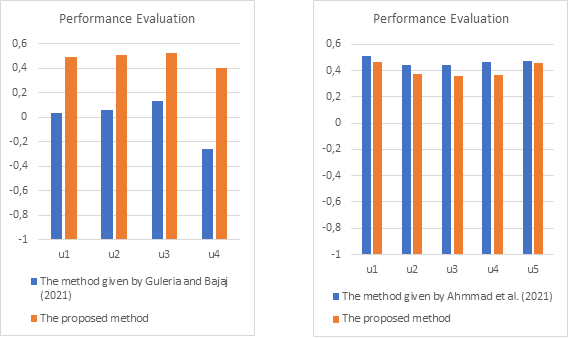
\includegraphics[scale=1]{graf1}
    \caption{Performance Evaluation\label{pe}}
    \label{fig:my_label}
\end{figure}
As a consequence of comparison, the proposed method  gives reliable and appropriate results. 



\begin{sidewaystable}[htbp]
\begin{center}\caption{Comparison the proposed method with the existing methods \label{co}} \footnotesize{
\begin{tabular}{c|c|c| c|  c}\hline
$\begin{array}{l} Methods\\given \\by
\end{array}$ & $\begin{array}{l} Alternatives/ \\ Attributes
\end{array}$ & Decision Matrices  & $\begin{array}{l} Results ~by \\existing\\ methods
\end{array}$ & $\begin{array}{l} Results ~by \\proposed\\ method
\end{array}$ \\
\hline $\begin{array}{l} Perveen \\ et~al.\cite{per}
\end{array}$ &  $\begin{array}{l} U=\{u_1, ...,u_7\}\\A=\{e_1, ...,e_5\}
\end{array}$  & $\left(
\begin{array}{c c c c c}
<0.8,0.1,0.4> &<0.5,0.2,0.6>&<0.7, 0.15, 0.3>&<0.6, 0.25,
0.31>&<0.55, 0.12, 0.5>
\\  <0.9, 0.1,0.3>&<0.7, 0.2,0.45>&<0.55,0.03, 0.12>&<0.65, 0.15, 0.56>&<0.8, 0.17, 0.3>\\
 <0.52, 0.02, 0.7>&<0.7, 0.12,0.31>&<0.45, 0.15, 0.5>&<0.6, 0.2, 0.4>&<0.75, 0.05,
 0.25>\\<0.7, 0.05, 0.4>&<0.45, 0.1, 0.55>&<0.56, 0.15,
 0.49>&<0.25, 0.05, 0.8>&<0.51, 0.1, 0.25>\\<0.7, 0.1,
 0.4>&<0.3, 0.2, 0.7>&<0.47, 0.25, 0.56>&<0.31, 0.15,
 0.6>&<0.8, 0.2, 0.4>\\<0.55,0.25, 0.65>&<0.81, 0.15,
 0.3>&<0.1, 0.2, 0.8>&<0.6, 0.05, 0.3>&<0.65,
 0.1,0.5>\\<0.92,0.1, 0.3>&<0.2, 0.25, 0.6>&<0.35, 0.2,
 0.7>&<0.8, 0.12, 0.4>&<0.75, 0.01, 0.3>
\end{array} \right)$ &   $\begin{array}{l} u_2>u_7\\>\{u_1, u_3,\\ u_4, u_6\}\\>u_5
\end{array}$   &  $\begin{array}{l} u_2
>u_7\\>u_1>u_3\\>u_5>u_6\\>u_4
\end{array}$ \\ \hline $\begin{array}{l} Yang\\ et ~al. \cite{yang}
\end{array}$ & $\begin{array}{l} U=\{u_1, ...,u_6\}\\A=\{e_1, ...,e_4\}
\end{array}$& $\left(
\begin{array}{c c c c}
<0.31,    0.22,    0.41>  &<0.54,    0.21,    0.15> & <0.6, 0.14,
0.26> &<0.38,    0.21,    0.4>
\\<0.12,    0.41,    0.33> & < 0.81,    0.11,    0.02> &  < 0.26,    0.51,    0.2> &< 0.65,    0.15,    0.18>\\
<0.23,    0.52, 0.21> & < 0.13,    0.48, 0.37> & < 0.72,    0.15,    0.03> &< 0.29,    0.58, 0.12>\\
 <0.45, 0.09,    0.36> &  < 0.23,    0.59, 0.18>  & <0.32, 0.49,    0.15> & <0.14, 0.32,    0.45>\\
 <0.57,    0.3,  0.05> &  <0.6, 0.23,    0.14> & <0.81,    0.11, 0.06> & < 0.43,    0.18,    0.35>\\
 <0.44, 0.4, 0.13>  &  < 0.42, 0.36, 022> &  < 0.43,    0.27,    0.13> &<
0.35, 0.29,    0.34>\end{array} \right)$
& $\begin{array}{l} u_5>u_2\\>\{u_1, u_3\}\\>\{u_4, u_6\}
\end{array}$  & $\begin{array}{l} u_5>u_1\\>u_2>u_3\\>u_6>u_4
\end{array}$  
\\ \hline $\begin{array}{l} Guleria \\ and\\ Bajaj\\ \cite{gul}
\end{array}$  & $\begin{array}{l} U=\{u_1, ...,u_4\}\\A=\{e_1, ...,e_4\}
\end{array}$ & $\left(
\begin{array}{c c c c}
<0.6,    0.2,    0.2>  &<0.5,    0.3,    0.2> & <0.5, 0.2,
0.3> &<0.2,    0.3,    0.4>
\\<0.4,    0.4,    0.3> & < 0.6,    0.3,    0.1> &  < 0.5,    0.3,    0.2> &< 0.7,    0.1,    0.2>\\
<0.2,    0.5, 0.4> & < 0.6,    0.3, 0.2> & < 0.7,    0.2,    0.2> &< 0.5,    0.3, 0.3>\\
 <0.6, 0.2,    0.3> &  < 0.2,    0.2, 0.6>  & <0.2, 0.3,    0.6> & <0.4, 0.2,    0.4>\end{array} \right)$
&  $\begin{array}{l} u_3>u_2\\>u_1>u_4
\end{array}$ & $\begin{array}{l} u_3>u_2\\>u_1>u_4
\end{array}$\\ \hline
  $\begin{array}{l} Ahmmad\\ et ~al. \cite{ah}
\end{array}$& $\begin{array}{l} U=\{u_1, ...,u_5\}\\A=\{e_1, ...,e_5\}
\end{array}$& $\left(
\begin{array}{c c c c c}
<0.7,    0.1,    0.2>  &<0.7,    0.1,    0.4> & <0.4, 0.4,
0.4> &<0.5,    0.6,    0.1>& <0.4, 0.4, 0.4>
\\<0.4,    0.3,    0.4> & < 0.5,    0.6,    0.4 > &  < 0.5,    0.4,    0.6> &< 0.4,    0.5,    0.3> & <0.2, 0.6, 0.5>\\
<0.5,    0.5, 0.3> & < 0.5,    0.5, 0.7> & < 0.2,    0.7,    0.3> &< 0.1,    0.7, 0.5> & <0.3, 0.4, 0.5>\\
 <0.3, 0.3,    0.6> &  < 0.5,    0.5, 0.5>  & <0.2, 0.8,    0.1> & <0.3, 0.6,    0.2> &<0.5,0.6, 0.3>\\
 <0.6,    0.1,  0.4> &  <0.4, 0.3,    0.6> & <0.9,    0.2, 0.2> & < 0.5,    0.5,    0.4> & <0.4, 0.7, 0.4>\end{array} \right)$ & $\begin{array}{l} u_1>u_5\\>u_4>u_2\\>u_6>u_3
\end{array}$ & $\begin{array}{l} u_1>u_5\\>u_2>u_4\\>u_6>u_3
\end{array}$ \\ \hline
\end{tabular}}\end{center}
\end{sidewaystable}





















\section{Conclusion}
In this paper, the soft set theory is extended by considering
spherical fuzziness to handle the uncertainty and to make them
more functional for solving multi-criteria decision-making problems. We first
introduced the new spherical fuzzy soft set theory with their
operations, then we represented a spherical fuzzy soft aggregation
operator to use them for constructing an algorithm to apply to the multi-criteria
decision-making procedure. Finally giving a numerical example to
demonstrate the applicability of this method, we compare the
results of this method with the methods given in \cite{ah, gul, per, yang}. But it can be remarked as the proposed theory is unable to capture two-dimensional information so it does not carry any information about the two-dimensional data especially physical problems. For
future work, we aim to extend the sfs-sets theory to the complex sfs-sets theory and apply this to the problems contains two-dimensional information. Also, we plan to study different kinds of aggregation operators to solve the
related problems to the (complex) spherical fuzzy soft environment.








\section*{Acknowledgement}
The authors are thankful to the
anonymous referees for their valuable suggestions.\\



\begin{thebibliography}{1}
\bibitem{ah} J. Ahmmad, T. Mahmood, R. Chinram, A. Iampan, {\it Some average aggregation operators based on spherical fuzzy soft sets and their applications in multi-criteria decision making}, AIMS Mathematics, {\bf 6(7)} (2021), 7798-7832.

\bibitem{as2} S. Ashraf, S. Abdullah, {\it Spherical aggregation operators and their
application in multiattribute group decision-making}, International
Journal of Intelligent Systems, {\bf 34(3)} (2019), 493-523.

\bibitem{as0} S. Ashraf, S. Abdullah, M. Aslam, M. Qiyas, M. A. Kutbi,
 {\it Spherical fuzzy sets and its representation of spherical fuzzy t-norms and t-conorms},
  Journal of Intelligent and Fuzzy Systems, {\bf 36(6)} (2019), 6089-6102.

\bibitem{as3} S. Ashraf, S. Abdullah, T. Mahmood, {\it Spherical fuzzy Dombi aggregation
operators and their application in group decision-making problems},
Journal of Ambient Intelligence and Humanized Computing, {\bf 11} (2020),
2731-2749.

\bibitem{as00} S. Ashraf, S. Abdullah, T. Mahmood, F. Ghani, T. Mahmood, {\it Spherical
fuzzy sets and their applications in multi-attribute decision
making problems}, Journal of Intelligent and Fuzzy Systems, {\bf 36(3)} (2019),
2829-2844.


\bibitem{ata} K. T. Atanassov, {\it Intuitionistic fuzzy sets}, Fuzzy Sets and
Systems, {\bf 20(1)} (2003), 87-96.


\bibitem{aa} A. Ayg\"{u}no\u glu, H. Ayg\"{u}n, {\it Some notes on soft topological spaces}, Neural Computing and Applications, {\bf 21(1)} (2012), 113-119.

\bibitem{babit} K. V. Babitha, S. J. John, {\it Hesitant fuzzy soft sets}, Journal of New Results in Science, {\bf 2(3)} (2013).

\bibitem{bel} R. Bellman, L. A. Zadeh, {\it Decision-making in a fuzzy
environment}, Manage Science, {\bf 17(3)} (1970).



\bibitem{cuon} B. Cuong, {\it Picture fuzzy sets-first results},  Seminar on
Neuro-fuzzy Systems with Applications Institute of Mathematics,
Hanoi, (2013).

\bibitem{cag} N. \c{C}a\u gman, S. Engino\u glu,  F. \c{C}\i tak, {\it Fuzzy soft set theory and its applications}, Iranian Journal of Fuzzy Systems, {\bf 8(3)} (2011), 137-147.

\bibitem{cag1}  N. \c{C}a\u gman, S. Karata\c s,  {\it Intuitionistic fuzzy soft set theory and its decision making}, Journal of Intelligent and Fuzzy Systems, {\bf 24(4)} (2013), 829-836.

\bibitem{cet} V. \c{C}etkin, A. Ayg\"{u}no\u glu, H. Ayg\"{u}n, {\it A new approach in handling soft
decision making problems}, Journal of Nonlinear Science and
Applications, {\bf 9} (2016), 231-239.

\bibitem{2s} V. \c{C}etkin, E. G\"{u}ner, H. Ayg\"{u}n,  {\it On 2S-metric spaces}, Soft Computing, {\bf 24(17)} (2020), 12731-12742.

\bibitem{gari} J. M. Garibaldi, T. Ozen, {\it Uncertain fuzzy reasoning: A case study in modelling
expert decision making},  IEEE Transactions on Fuzzy Systems,
{\bf 15(1)} (2007), 16-30.

\bibitem{gul} A. Guleria, R. K. Bajaj, {\it T-spherical fuzzy soft sets and its aggregation operators with application in decision-making}, Scientia Iranica, {\bf 28(2)} (2021), 1014-1029.

\bibitem{gun} E. G\"{u}ner, H. Ayg\"{u}n, {\it Generalized spherical fuzzy Einstein aggregation operators: Application to multi-criteria group decision-making problems}, Conference Proceedings of Science and Technology, {\bf 3(2)} (2020), 227-235.
 
\bibitem{jin} Y. Jin, S. Ashraf, S. Abdullah, {\it Spherical fuzzy logarithmic
aggregation operators based on entropy and their application
indecision support systems}, Entropy, {\bf 21(7)} (2019), 628-664.

\bibitem{kut0} C. Kahraman, F. Kutlu G\"{u}ndo\u gdu, {\it From 1D to 3D membership: Spherical fuzzy
sets}, BOS/SOR2018 Conference, Warsaw, Poland, (2018).

\bibitem{kutlu} F. Kutlu G\"{u}ndo\u gdu, C. Kahraman, {\it A novel VIKOR method using spherical
fuzzy sets and its application to warehouse site selection}, Journal
of Intelligent and Fuzzy Systems, {\bf 37(1)} (2019), 1197-1211.

\bibitem{kutlu1} F. Kutlu G\"{u}ndo\u gdu, C. Kahraman, {\it Extension of WASPAS with spherical
fuzzy sets}, Informatica, {\bf 30(2)} (2019), 269-292.

\bibitem{kutlu2} F. Kutlu G\"{u}ndo\u gdu, C. Kahraman, {\it Spherical fuzzy sets and spherical
fuzzy TOPSIS method}, Journal of Intelligent and Fuzzy Systems,
{\bf 36(1)} (2019), 337-352.

\bibitem{mah} T. Mahmood, U. Kifayat, Q. Khan, N. Jan, {\it An approach toward decision
making and medical diagnosis problems using the concept of
spherical fuzzy sets}, Neural Computing and Applications, {\bf 31} (2018),
7041-7053.


\bibitem{maj} P. K. Maji, R. Biswas, A. R.  Roy, {\it Fuzzy soft sets}, Journal of Fuzzy Mathematics, {\bf 9(3)} (2001), 589-602.

\bibitem{maji1} P. K. Maji, R. Biswas, A. R. Roy, {\it Soft set theory}, Computers Mathematics
with Applications, {\bf 45} (2003), 555-562.

\bibitem{maji} P. K. Maji, A. R. Roy, {\it An application of soft set in decision making
problem}, Computers Mathematics with Applications, {\bf 44} (2002), 1077-1083.


\bibitem{mol} D. Molodtsov, {\it Soft set theory-first results}, Computers Mathematics
with Applications, {\bf 37} (1999), 19-31.



\bibitem{pazar} B. Pazar Varol, H. Ayg\"{u}n, {\it Fuzzy soft topology}, Hacettepe Journal of
Mathematics and Statistics, {\bf 41(3)} (2012), 407-419.

\bibitem{peng} X. Peng, Y. Yang, J. Song, Y. Jiang, {\it Pythagorean fuzzy soft set and
its application}, Computer Engineering, {\bf 41} (2015), 224-229.


\bibitem{per} P. F. A. Perveen, J. J. Sunil, K. Babitha, H. Garg,
{\it Spherical fuzzy soft sets and its applications in decision-making
problems}, Journal of Intelligent and Fuzzy Systems, {\bf 37(6)} (2019),
8237-8250.


\bibitem{sam} R. Sambuc, {\it Function $\Phi$-flous application al faide au diagnostic en pathologie
thyroidienne}, University of Marseille, (1975).

\bibitem{sel} G. Selvachandran, H. Garg, S. G. Quek, {\it Vague entropy measure for complex vague soft sets}, Entropy, {\bf 20(6)} (2018), 403.

\bibitem{sma} F. Smarandache, {\it Neutrosophy: Neutrosophic Probability, Set and Logic: Analytic
Synthesis and Synthetic Analysis}, (1998).

\bibitem{tor} V. Torra, {\it Hesitant fuzzy sets}, International Journal of Intelligent Systems, {\bf 25(6)} (2010), 529-539.

\bibitem{wan} L. Wang, H. Garg, N. Li, {\it Pythagorean fuzzy interactive Hamacher power aggregation operators for assessment of express service quality with entropy weight}, Soft Computing, {\bf 25(2)} (2021), 973-993.

\bibitem{wei} G. Wei, {\it Picture fuzzy aggregation operators and their application
to multiple attribute decision making}, Journal of Intelligent and
Fuzzy Systems, {\bf 33(2)} (2017), 713-724.

\bibitem{wei1} G. Wei, {\it Picture fuzzy Hamacher aggregation operators and their
application to multiple attribute decision making}, Fundamenta
Informaticae, {\bf 157(3)} (2018), 271-320.

\bibitem{wes} G. M Weiss, K. Yoneda, T. Hayajneh, {\it Smartphone and smartwatch-based biometrics using activities of daily living}, IEEE Access, {\bf 7} (2019), 133190-133202.


\bibitem{xu} Z. S. Xu, {\it Intuitionistic fuzzy aggregation operators}, IEEE Transactions on Fuzzy Systems, {\bf 15(6)} (2007), 1179-1187.


\bibitem{yager} R. Yager, {\it On the theory of bags}, International Journal of General Systems, {\bf 13(1)} (1986), 23-37.


\bibitem{yager1} R. R.  Yager, {\it Pythagorean fuzzy subsets}, Proceedings of Joint
IFSA World Congress and NAFIPS Annual Meeting, Edmonton, Canada,
(2013).

\bibitem{yang} Y. Yang, C. Liang, S. Ji, T. Liu, {\it Adjustable soft discernibility matrix based
on picture fuzzy soft sets and its applications in decision
making}, Journal of Intelligent and Fuzzy Systems, {\bf 29(4)} (2015),
1711-1722.

\bibitem{zadeh} L. A. Zadeh, {\it Fuzzy sets}, Information and Control, {\bf 8} (1965), 338-353.

\bibitem{zadeh1} L. A. Zadeh, {\it The concept of a linguistic variable and its
application to approximate reasoning}, Information Sciences, {\bf 8} (1975),
199-249.

\end{thebibliography}



\end{document}